% -*- LaTeX -*-

\documentclass[a4paper,twoside]{article}

% \usepackage[koi8-r]{inputenc}
\usepackage[T1]{fontenc}
\usepackage[american]{babel}
\usepackage[colorlinks,urlcolor=blue,unicode=true]{hyperref}
\usepackage{url}

\usepackage[pdftex]{graphics}
%\usepackage{pslatex}
% \usepackage[dvips,final]{epsfig}
% \usepackage{cm-super}
%\usepackage[colorlinks,urlcolor=blue]{hyperref}
%\usepackage{url}

\usepackage{rup}
%% Define a new 'leo' style for the package that will use a smaller font.
\makeatletter
\def\url@leostyle{%
  \@ifundefined{selectfont}{\def\UrlFont{\sf}}{\def\UrlFont{\small\ttfamily}}}
\makeatother
%% Now actually use the newly defined style.
\urlstyle{leo}


\version{0.1}
\title{Use Case Specification: ``Unit Test Framework''}

\project{Exam}

\RevHistory{2007--03--08 & 1.0 & Initial document & Petr Ovtchenkov \cr \hline}

\begin{document}

\maketitle
% toc
\tableofcontents

\section{Unit Test Framework}

% [The following template is provided for a Use-Case
% Specification, which contains the textual properties of the use case.
% This document is used with a requirements management tool, such as Rational
% RequisitePro, for specifying and marking the requirements within the use case
% properties]

% [The diagrams of the use case can be developed in a visual
% modeling tool, such as Rational Rose. A use-case report (with all
% properties) may be generated with Rational SoDA.  For more information, see the tool mentors in the Rational
% Unified Process.]

\subsection{Brief Description}

% [The description should briefly convey the role and purpose
% of the use case.  A single paragraph
% should suffice for this description.]

Unit test framework should provide a matched set of components for writing
test programs, grouping tests into test cases and test suites,
monitoring and controlling their runtime execution. Unit test framework
should be convenient for testing programs and set of programs that implement
services and client--server technologies (the set of intercommunicating programs, many
control flows).

\section{Flow of Events}

\subsection{Basic Flow}

% [This use case starts when the actor does something.  An actor always initiates use Cases.  The use case should describe what the actor
% does and what the system does in response. 
% It should be phrased in the form of a dialog between the actor and the
% system.
%
% The use case should describe what happens inside the system,
% but not how or why.  If information is
% exchanged, be specific about what is passed back and forth.  For example, it is not very illuminating to
% say that the Actor enters customer information. It is better to say the Actor
% enters the customer's name and address. 
% A Glossary of Terms is often useful to keep the complexity of the use
% case manageable---you
% may want to define things like customer information there to keep the use case
% from drowning in details.
%
% Simple alternatives may be presented within the text of the
% use case.  If it only takes a few
% sentences to describe what happens when there is an alternative, do it directly
% within the \textbf{Flow of Events} section. 
% If the alternative flows are more complex, use a separate section to
% describe it.  For example, an \textbf{Alternative Flow}
% subsection explains how to describe more complex alternatives.
%
% A picture is sometimes worth a thousand words, though there
% is no substitute for clean, clear prose. 
% If it improves clarity, feel free to paste graphical depictions of user
% interfaces, process flows or other figures into the use case.  If a flow chart is useful to present a
% complex decision process, by all means use it! 
% Similarly for state-dependent behavior, a state-transition diagram often
% clarifies the behavior of a system better than pages upon pages of text.  Use the right presentation medium for your
% problem, but be wary of using terminology, notations or figures that your
% audience may not understand.  Remember
% that your purpose is to clarify, not obscure.]

The test suite with single control flow. It notify about start of test suite,
run tests within this test suite (in the order following from tests dependency
graph), report about checks of conditions (verbosity depends upon log level), and print the resulting summary of the test suite (see fig.\ref{SingleFlow}).

\begin{figure}
  \begin{center}
%  \input intercessor-time.pstex_t
%   \input p1.pdf_t
% \scalebox{0.8}{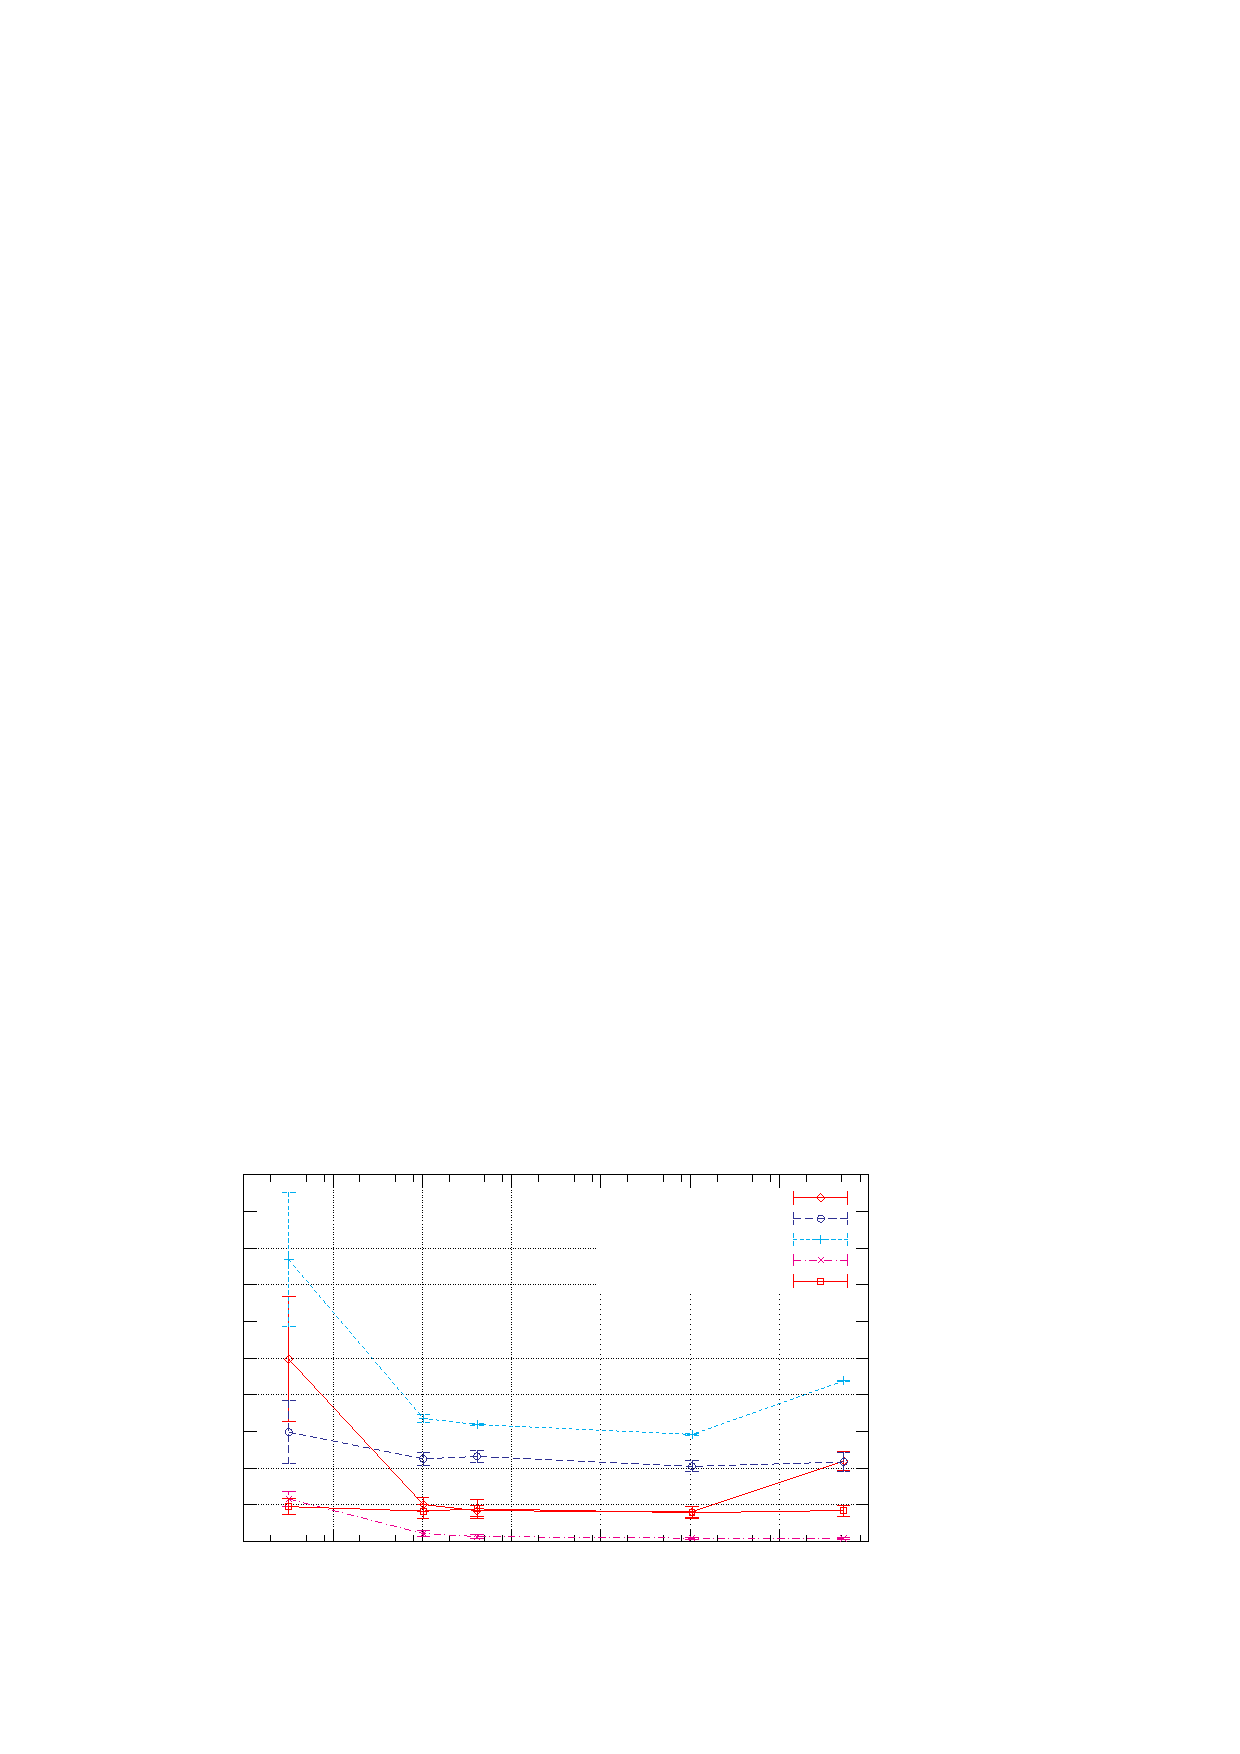
\includegraphics{p1.pdf}}
  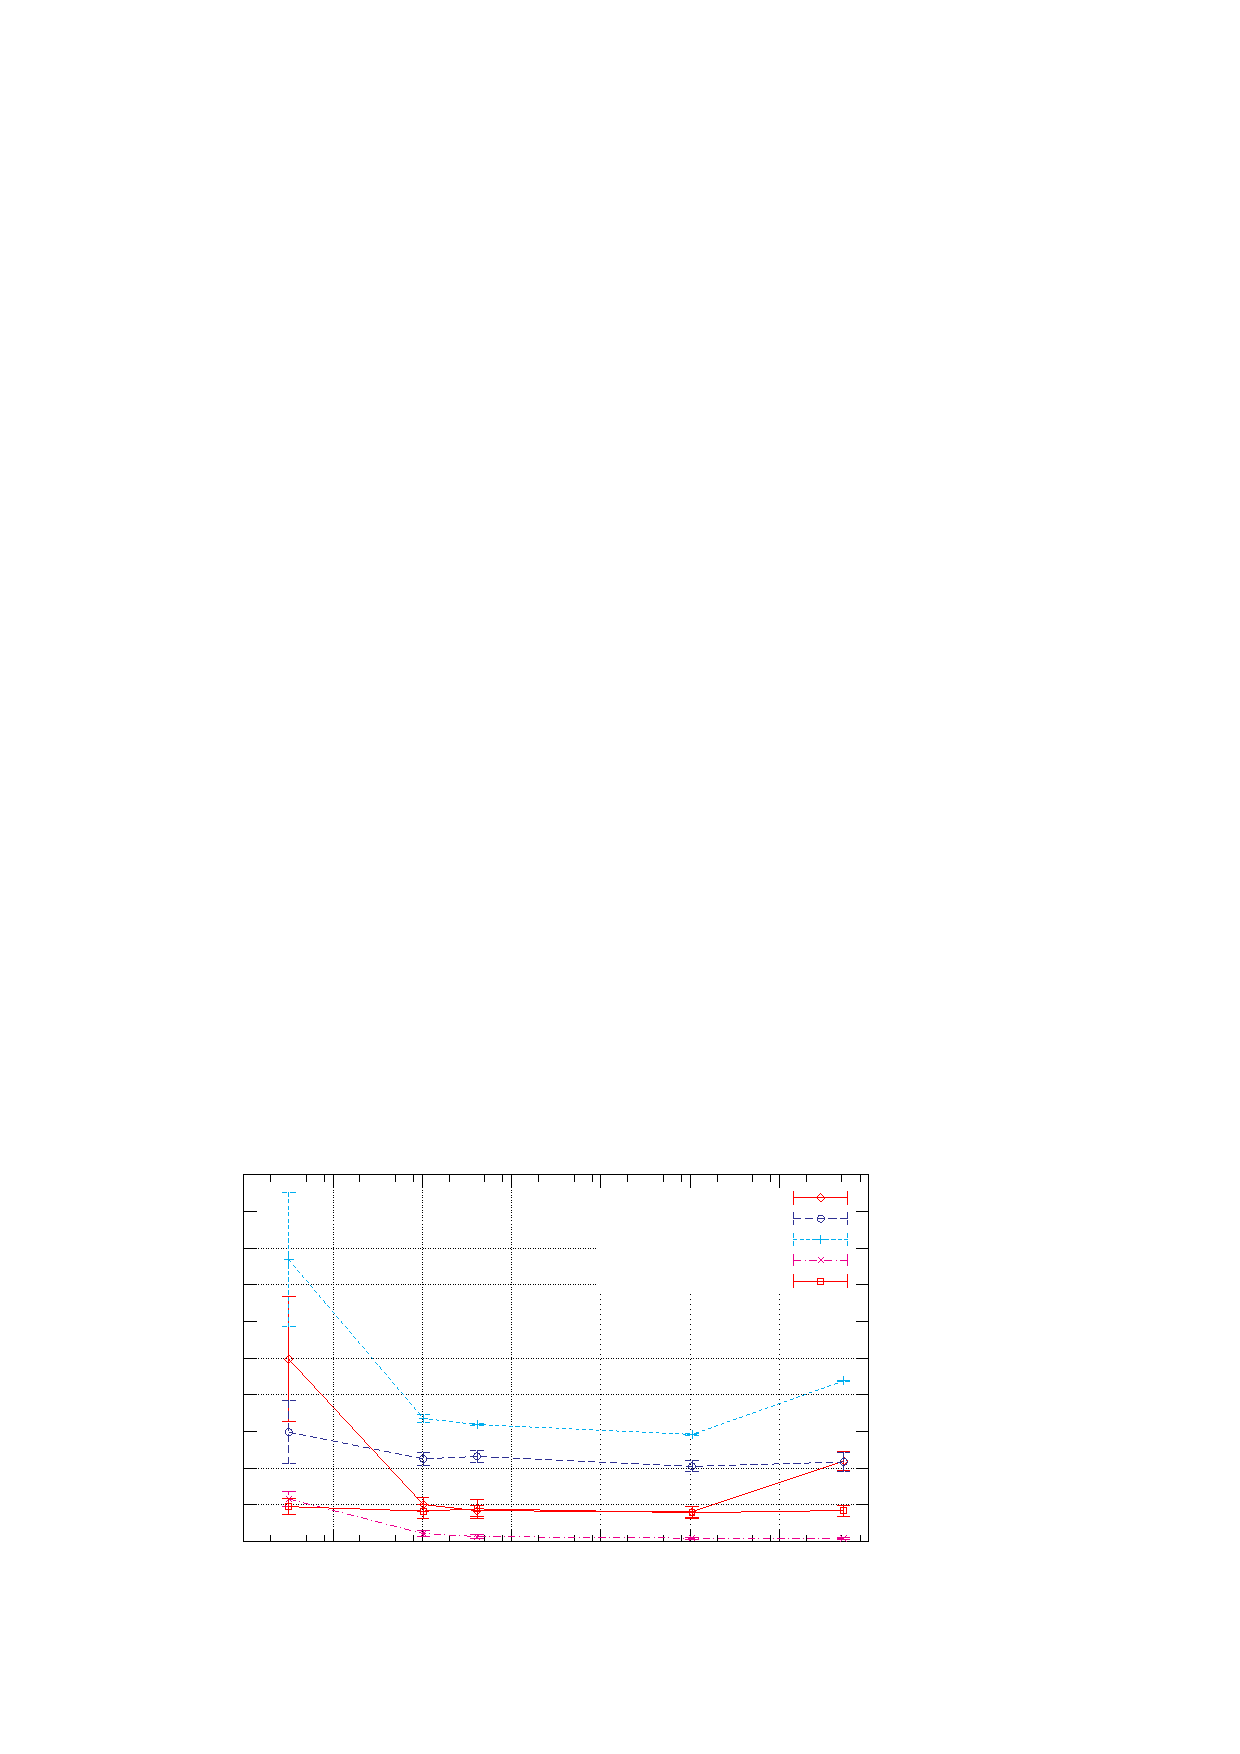
\includegraphics{p1.mps}
  \end{center}
  \caption{The test case with single control flow.\label{SingleFlow}}
\end{figure}


\subsection{Alternative Flows}

\subsubsection{Test suite for interactive program}

% [More complex alternatives should be described in a separate
% section, which is referred to in the \textbf{Basic Flow} subsection
%  of \textbf{Flow of Events} section.  Think of the 
% \textbf{Alternative Flow}> subsections like alternative behavior---each 
% alternative flow
% represents alternative behavior, many times because of exceptions that occur in
% the main flow.  They may be as long as
% necessary to describe the events associated with the alternative behavior.  When an alternative flow ends, the events of
% the main flow of events are resumed unless otherwise stated.]

The test suite with single control flow. It notify about start of test suite,
run tests within this test suite (in the order, described by tests dependency
graph), print conditions report (verbosity depends upon log level), and print the resulting summary of the test suite (see fig.\ref{InteractiveSingleFlow}).
During execution of the test suite, it require interaction with: it print
messages onto terminal and expect input from terminal.

\begin{figure}
  \begin{center}
  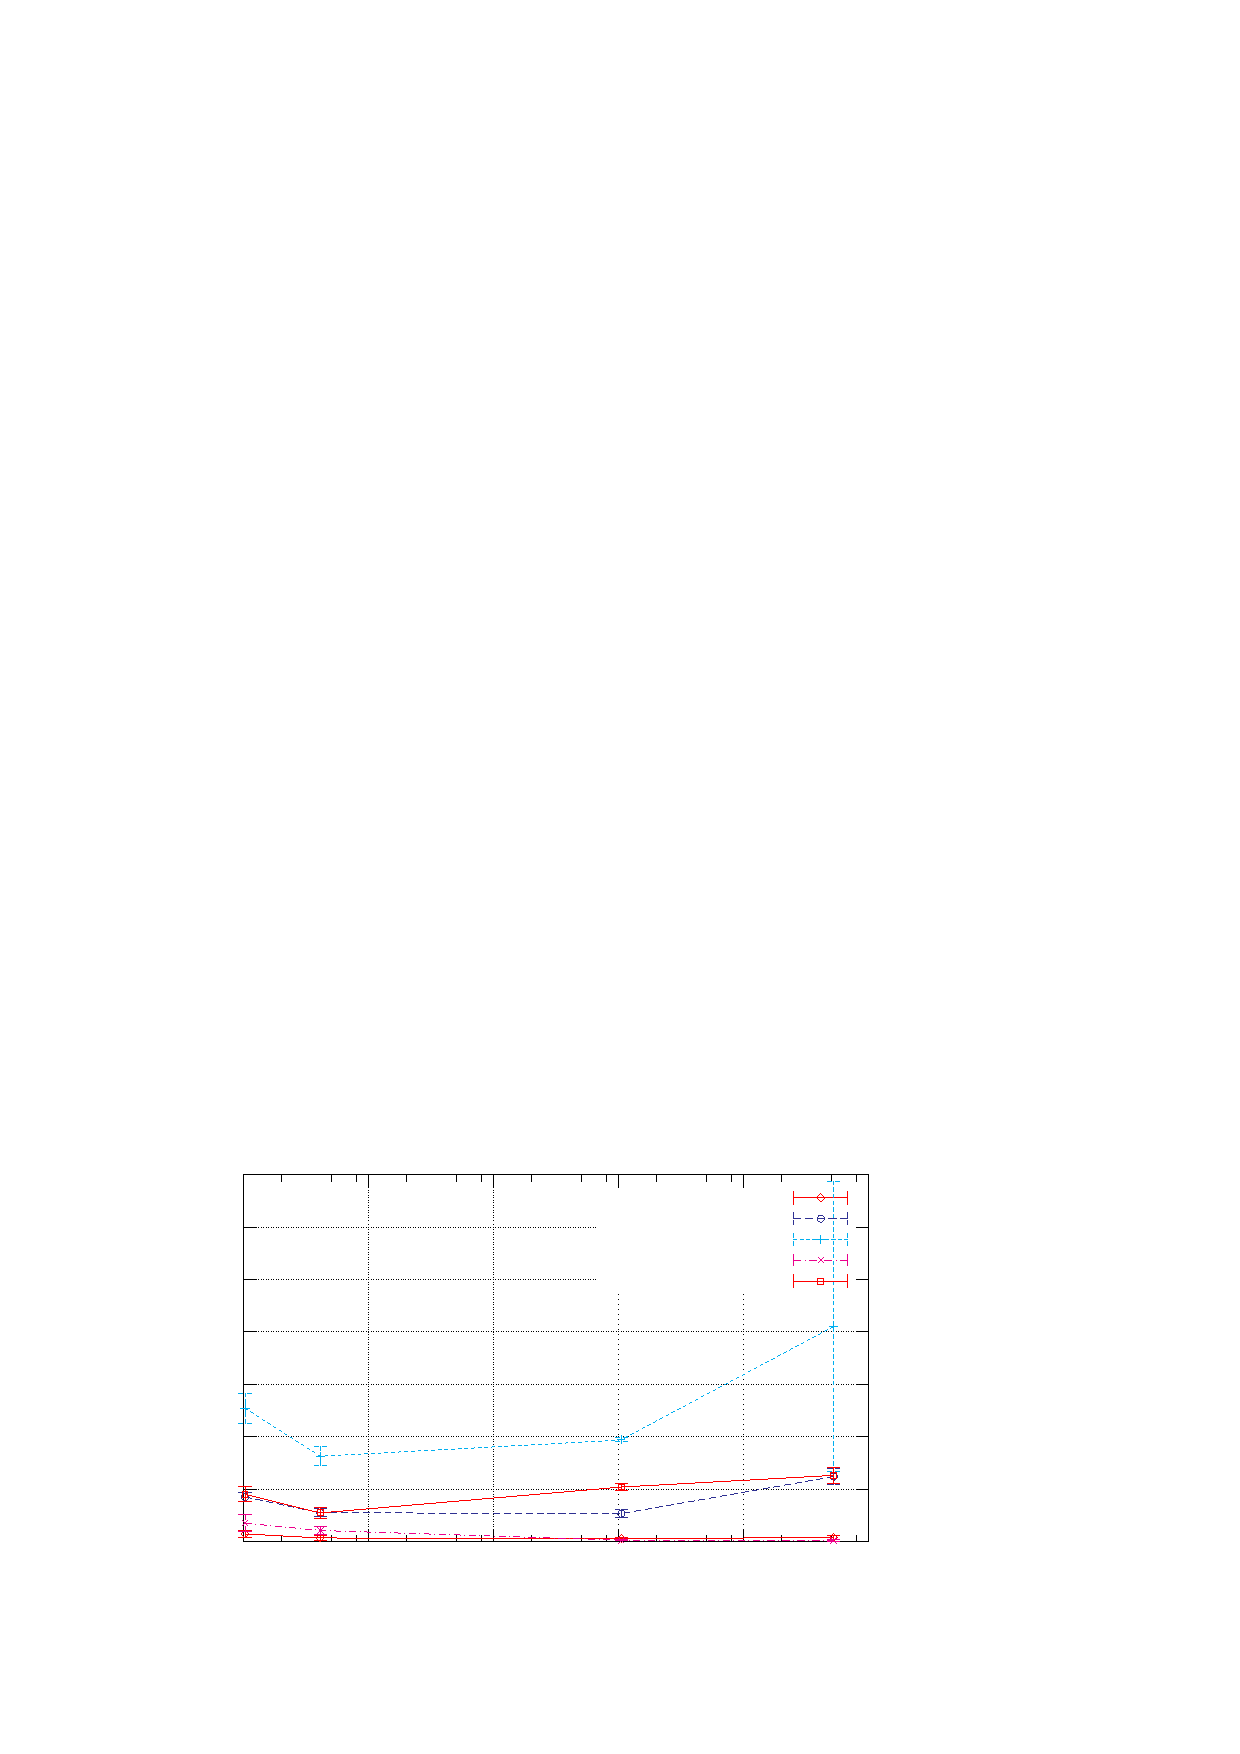
\includegraphics{p5.mps}
  \end{center}
  \caption{The test case with single control flow; test suite is
           interactive, it print some message to terminal and expect input
           from terminal.\label{InteractiveSingleFlow}}
\end{figure}

This use-case reflect test suite for interactive part of program.

\subsubsection{Multi-threaded test suite}

% [There may be, and most likely will be, a number of
% alternative flows in a use case.  Keep
% each alternative separate to improve clarity. 
% Using alternative flows improves the readability of the use case, as
% well as preventing use cases from being decomposed into hierarchies of use
% cases.  Keep in mind that use cases are
% just textual descriptions, and their main purpose is to document the behavior
% of a system in a clear, concise, and understandable way.]

The test suite with more then one control flow. It register start of test suite,
run tests within this test suite (in the order, described by tests dependency
graph), print conditions report (verbosity depends upon log level), and print the resulting summary of the test suite (see fig.\ref{ThreadedFlow}).
Test control flow is splitted into few threads.

\begin{figure}
  \begin{center}
  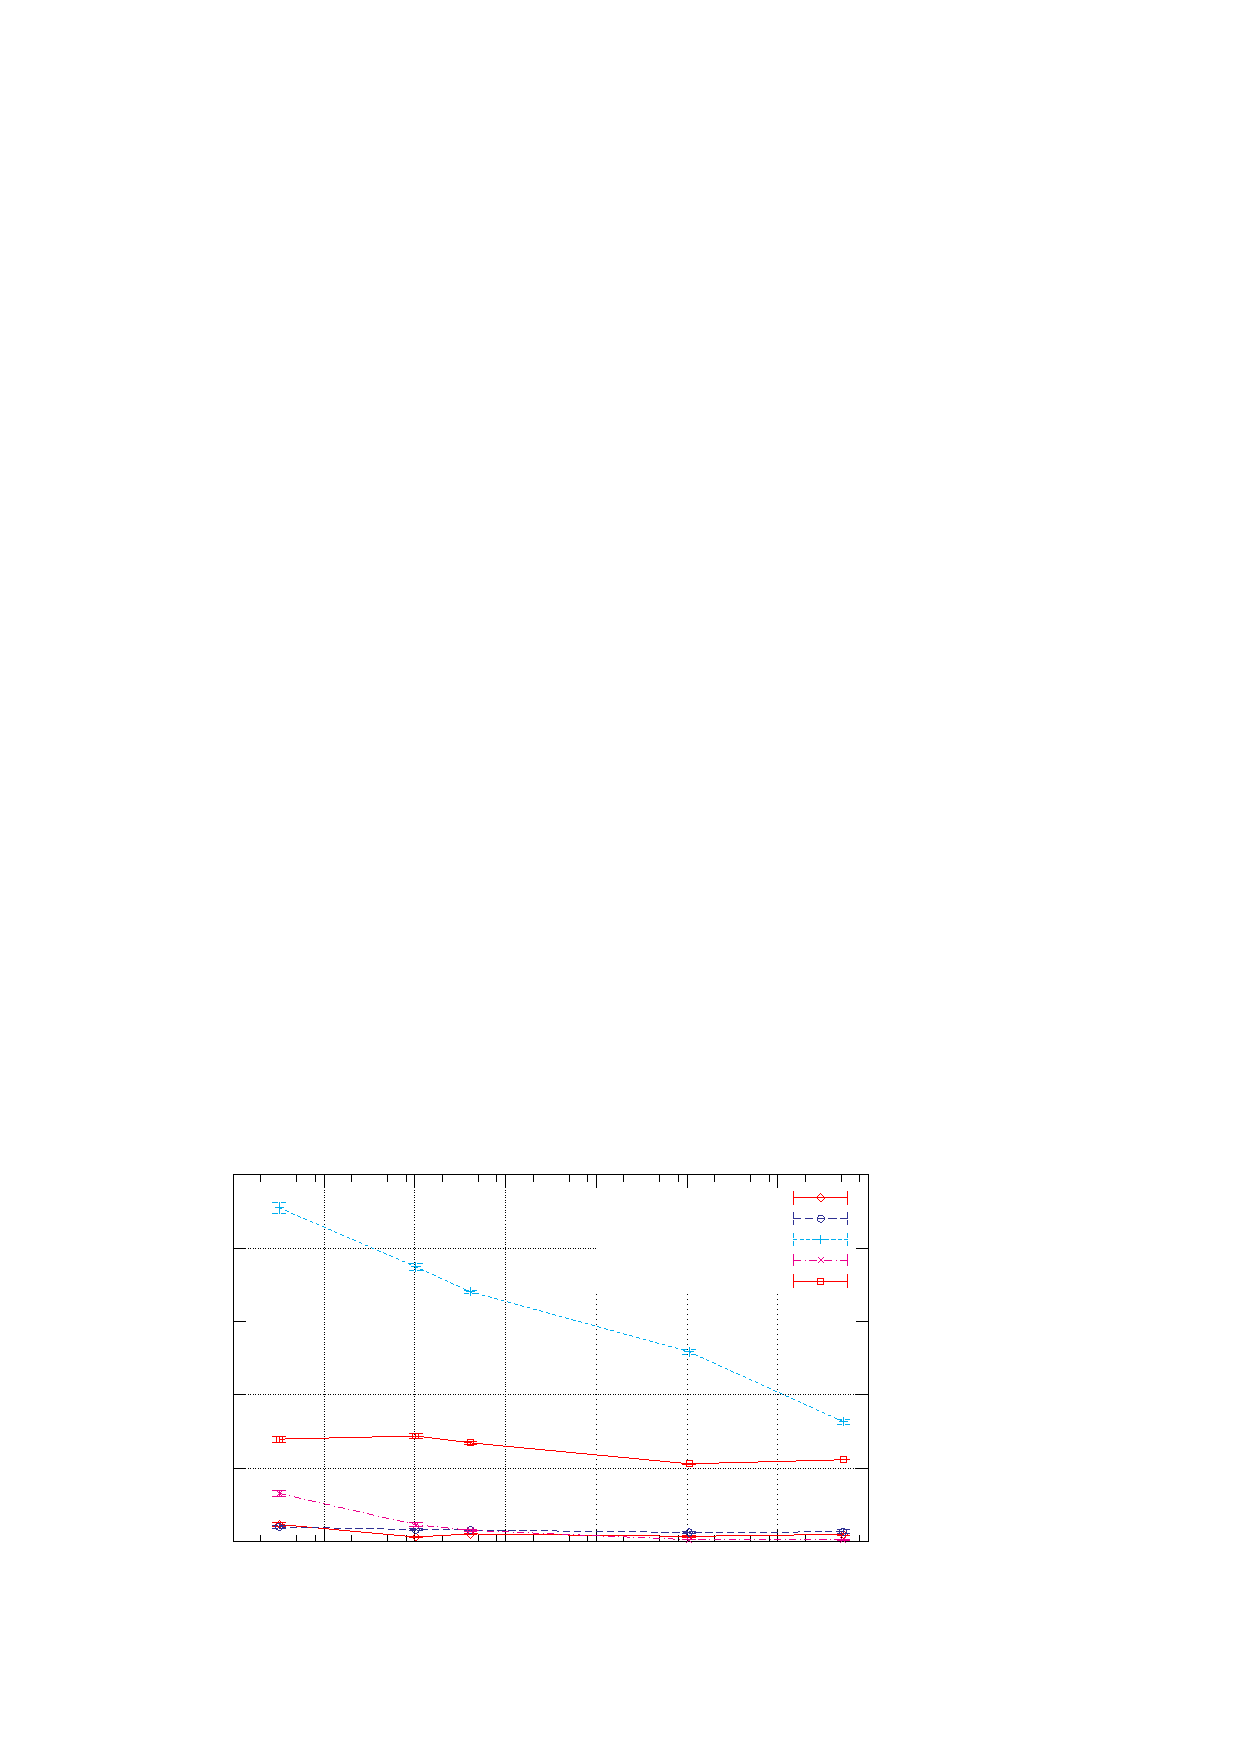
\includegraphics{p2.mps}
  \end{center}
  \caption{The test case with few control flows, single process.\label{ThreadedFlow}}
\end{figure}

This use-case reflect test suite for multi-threaded program, such as server,
that provide some kind of service.

\subsubsection{Test suite with fork}

The test suite with more then one control flow. It register start of test suite,
run tests within this test suite (in the order, described by tests dependency
graph), print conditions report (verbosity depends upon log level), and print the resulting summary of the test suite (see fig.\ref{ForkedFlow}).
Some tests of the test suite forked into several processes.

\begin{figure}
  \begin{center}
  \includegraphics{p4.mps}
  \end{center}
  \caption{The test case with few control flows, process forked.\label{ForkedFlow}}
\end{figure}

This use-case reflect test suite for daemons and client-server interaction.

\subsubsection{Test suite with process intercommunication}

The test suite with more then one control flow. It register start of test suite,
run tests within this test suite (in the order, described by tests dependency
graph), print conditions report (verbosity depends upon log level), and print the resulting summary of the test suite (see fig.\ref{IntercomProcesses}).
Some tests of the test suite forked into several processes.

\begin{figure}
  \begin{center}
  \includegraphics{p3.mps}
  \end{center}
  \caption{The test case with few control flows, intercommunicated processes.\label{IntercomProcesses}}
\end{figure}

This use-case reflect test suite for daemons and client-server interaction.

\section{Special Requirements}

% [A special requirement is typically a non-functional
% requirement that is specific to a use case, but is not easily or naturally
% specified in the text of the use case's event flow. Examples of special
% requirements include legal and regulatory requirements, application standards,
% and quality attributes of the system to be built including usability,
% reliability, performance or supportability requirements. Additionally, other
% requirements---such
% as operating systems and environments, compatibility requirements, and design
% constraints---should be captured in this section.]

\subsection{Suitable for debugging}

\begin{figure}
  \begin{center}
  \includegraphics{debug-focus.mps}
  \end{center}
  \caption{Development application: functionality implementation cycle.\label{DevCycle}}
\end{figure}

Unit tests not only instrument of QA (see fig.~\ref{DevCycle}).
Unit tests written
in parallel with functionality implementation,\footnote{as assume XP technique}
provide a good practice ground
for debugging. Implementation of special test cases for debugging
after detection problem in unit test isn't a good idea by financial (time and other resources) reasons.
Even more: in non-trivial cases not evident, what was wrong:
either incorrect functionality imlementation, or test, or even
specification. Developer should has a chance to debug program
keeping in mind as main functionality, as unit test logic.

Due to this unit test framework intended for testing services, and services
often has own logic of signal processing, the unit test framework
should not (at least by default) intervenes into signal catching.
This also concern fatal errors with dumping core: dumping core ``as is''
is more preferable way (useful for post-mortal debugging) then nice report
``you test died'' with unuseful stack.

\subsection{Output from few control flows}

Unit test suite should provide reasonable output as for tests
with single control flow, as for multi-threaded and multi-process tests.

Unit test suite should provide reasonable output for test
with console output and input, i.e. split prints from interaction with user
from prints about failed conditions.

\subsection{Integrable}

To be light-weight, easy integrable into other tools and scripts.

\subsection{Tests dependency\label{TestDependency}}

Tests run order should be determined from tests dependency graph.

\subsection{Tests grouping}

The ability of grouping tests is desirable:
\begin{itemize}
  \item single function tests
  \item class (group of tests) with initialization and finalization.
\end{itemize}

\subsection{Report format}

Unit test framework should provide few levels of output verbosity, and
few formats of reports (plain text, xml/html).

\subsection{Test timeout}

Due to deadlock (or other conditions, leads to stalled test) may occur,
it would be nice if monitoring program abort such test after specified timeout,
and continue other tests (taken into account tests dependencies, section~\ref{TestDependency}).

% \section{Pre-Conditions}

% [A pre-condition of a use case is the state of the system
% that must be present prior to a use case being performed.]

% \subsection{Pre-condition One}

% \section{Post-Conditions}

% [A post-condition of a use case is a list of possible states
% the system can be in immediately after a use case has finished.]

% \subsection{Post-condition One}

\section{Extension Points}

% [Extension points of the use case.]

\subsection{Remote testing}

% [Definition of the location of the extension point in the
% flow of events.]

Test suite monitoring may be performed from remote host. This also useful
if test suite allow monitoring a few (intercommunicating) processes, that
run on different hosts.

\subsection{Performance Mesure}

Unit tests may be used for performance measure of key technology solutions.

%\bibliographystyle{plain}
%\bibliography{db-res}

\end{document}
